\documentclass[12pt,spanish]{article}

% aprovechamiento de la p\'agina -- fill an A4 (210mm x 297mm) page
% Note: 1 inch = 25.4 mm = 72.27 pt
% 1 pt = 3.5 mm (approx)

% vertical page layout -- one inch margin top and bottom
\topmargin      -10 mm   % top margin less 1 inch
\headheight       0 mm   % height of box containing the head
\headsep          0 mm   % space between the head and the body of the page
\textheight     255 mm   % the height of text on the page
\footskip         7 mm   % distance from bottom of body to bottom of foot

% horizontal page layout -- one inch margin each side
\oddsidemargin    0 mm     % inner margin less one inch on odd pages
\evensidemargin   0 mm     % inner margin less one inch on even pages
\textwidth      159 mm     % normal width of text on page

\usepackage{babel}
\usepackage[utf8]{inputenc}
\usepackage{amsmath,amsthm,mathtools}
\usepackage{amsfonts,amssymb,latexsym}
\usepackage{enumerate}
\usepackage[dvips,usenames]{color}
\definecolor{RojoAnayelRey}{rgb}{1,.25,.25}
\usepackage[bookmarks=true,
            bookmarksnumbered=false, % true means bookmarks in 
                                     % left window are numbered                         
            bookmarksopen=false,     % true means only level 1
                                     % are displayed.
            colorlinks=true,
            linkcolor=webred]{hyperref}
\definecolor{webgreen}{rgb}{0, 0.5, 0} % less intense green
\definecolor{webblue}{rgb}{0, 0, 0.5}  % less intense blue
\definecolor{webred}{rgb}{0.5, 0, 0}   % less intense red
\definecolor{dkgreen}{rgb}{0,0.6,0}
\definecolor{gray}{rgb}{0.5,0.5,0.5}
\definecolor{mauve}{rgb}{0.58,0,0.82}
\definecolor{MistyRose}{RGB}{255,228,225}
\definecolor{LightCyan}{RGB}{224,255,255}

\usepackage[T1]{fontenc}

% Entorno para estilo de ejercicios
\newenvironment{ejercicio}[1]{\textbf{#1} \vspace*{5mm}}{\vspace*{5mm}}
\setlength{\parindent}{9pt} 

% uso de imágenes

\usepackage{graphicx}
\graphicspath{ {images/} }


\begin{document}


\title{Estructura de Computadores - Práctica 2}
\author{Yábir García Benchakhtir}
\date{\today}
\maketitle



\section*{Preguntas de autocombración: suma\_08\_Casm}

\begin{ejercicio}{1. Obtener el código de ensamblador generado con gcc
    y compararlo con el anterior de \textit{suma\_08} ¿Qué diferencias
    hay?}

  Como principal diferencia encontramos que el código generado por ensamblador combrueba que la lista sea no vacía. También podemos destacar que en lugar de usar \textbf{inc} utiliza \textbf{addl}.
\end{ejercicio}

\begin{ejercicio}{2. Comparar el cód digo generado comentando
    \textit{cc} y descomentando \textit{cc} de la lista clobber.  ¿Hay
    alguna diferencia?}
  
  Haciendo la compilación con la orden \textit{gcc -S suma\_08\_Casm.c
    -o suma8.s -m32 -fno-omit-frame-pointe} y usando la orden
  \textit{diff} no hay ninguna diferencia.
\end{ejercicio}

\begin{ejercicio}{3. No necesitamos declarar ningún otro sobreescrito, pero por un motivo distinto que en el ejemplo anterior. ¿Por qué?}

  No necesitamos ninguna restricción extra porque los registros están
  puestos por gcc. Lo hacemos así ya que necesitamos acceder a los
  valores proporcionados a la función.
  
\end{ejercicio}

\begin{ejercicio}{4. Si res es una variable de salida ¿por qué se le ha
    indicado restricción \textit{+r} en lugar de \textit{=r}?}

  Necesitamos marcarlo con la opción de escritura ya que al usar add
  estamos modificando su valor.
  
\end{ejercicio}

\begin{ejercicio}{5. Explicar por qué en este caso se prefiere acabar la linea en \textit{\textbackslash n} en lugar de \textit{\textbackslash n \textbackslash t}}

  Cuando usamos \textit{(\textbackslash n \textbackslash t} lo hacemos para indentar la siguiente
  linea e indicar estructuras que dependen de otras. En este caso
  tenemos una única linea y las instrucción siguiente no van a
  depender de eta.
  
\end{ejercicio}

\section*{Preguntas de autocombración: suma\_09\_Casm}

\begin{ejercicio}{1. Repasar el código de ensamblador generado por gcc
    para las tres versiones. ¿Hay alguna diferencia?}

  En \textit{suma\_09} la función suma2 se corresponde con la de suma\_08
  y la función suma3 con la de suma\_07. Sus códigos ensambladores son
  casi identicos. 
  
\end{ejercicio}

\begin{ejercicio}{2. En la versión 3 se ha añadido un clobber que antes
    no estaba (ver Figura 10). ¿Acaso no sirve para nada ese clobber?
    ¿No hay diferencias en el código en ensamblador generado?}

  La diferencia más notoria es que en suma\_09 se hace \textit{pushl
    \% ebx}. Con lo cual está salvando su contenido y por lo tanto se
  está preocupando de salvar el contenido de cara a otras funciones
  que puedan usar su contenido.
  
\end{ejercicio}

\begin{ejercicio}{3. En la versión 3 se han escrito los registros
    con dos símbolos \%, en lugar de uno (como en la Figura 10).
    ¿Qué pasa si se escriben como antes? ¿Por qué no pasaba eso
    antes?}

  Escribimos ahora doble porcentaje porque en los clobber hemos puesto
  \textit{ebx} y para indicarle a gcc que nos referimos al registro y
  no al clobber ponemos el doble porcentaje.
  
\end{ejercicio}

\begin{ejercicio}{4. ¿Cuántos elementos tiene el array? ¿Cuánta memoria
    ocupa? ¿Cuánto vale la suma? ¿Cómo se llaman ese tipo de sumas?
    ¿Qué fórmula se usa para calcular una suma como esa?}

  Como estamos desplazando un \textit{1} 16 posiciones a la izquiera
  el tamaño del array será de $2^{16}$. Como lo estamos definiendo
  como un array de \textit{int} y suponiendo que este tipo de dato usa
  $4B$ el tamaño del array será $4*2^{16} = 2^{18}$. El valor de la suma es 2147516416 y se calcula sabiendo que se trata de una progresión aritmética:

  $$\sum_{i=0}^{2^{16}}i = \frac{n(a_1 + a_n)}{2}$$

  donde $n$ es el número total de términos, $a_1$ es el primer término
  de la sucesión y $a_n$ es el último término.
  
\end{ejercicio}

\begin{ejercicio}{5. El código C imprime un mensaje diciendo
    $\frac{N\cdot (N+1)}{2}$, pero luego calcula $\frac{(SIZE-1)\cdot
      SIZE}{2}$. ¿Cuál es la fórmula correcta?}

  Ambas son correctas porque en el caso de que este lleno $SIZE = N+1$
  y usando la igualdad del ejercicio anterior ambas formulas son
  iguales.
  
\end{ejercicio}

\newpage

\begin{ejercicio}{6. Esa línea viene comentada con /* OF */. ¿Qué
    puede significar ese comentario?  ¿Qué se puede decir acerca
    de la forma de escribir esa fórrmula? Si es por ``incomodida
    para calcular la fórmula'', ¿qué se podría haber hecho para evitar
    de golpe cualquier incomodidad? ¿Cómo se escribiría
    entonces, más cómodamente, la fórmula, y tooda la instrucción
    printf?}

  Puede significar que se produzca un overflow ya que estamos
  calculando un número que es del orden de $2^{32}$. Para solucionar
  esto podemos usar tipos de datos que permitan almacenar un mayor
  tamaño. Podríamos haber escrito la orden printf como:\\

  \textit{printf("\%lu \textbackslash n", SIZE*(SIZE-1)/2)}
  
\end{ejercicio}

\begin{ejercicio}{8. ¿Hay alguna manera de ganar a gcc haciendo el
    tipo de cosas que venimos haciendo con suma?}

  Por lo general no, aunque usando asm podemos obtener mejor
  rendimiento en algunos casos o cuando trabajamos con sistemas
  especiales que cuenten con un repertorio de instrucciones que el
  compilador no sepa manejar o no de manera optima.
\end{ejercicio}
\section*{Estudio sobre el rendimiento}
\section*{Cuestiones sobre popcount.c}

\begin{ejercicio}{1. xoDar una respuesta precisa a la primera pregunta
    (primer párrafo) de la Sección 4.1: en el peor caso, cuando todos
    los elementos tienen todos los bits activados... ¿cómo de grande
    puede ser N sin que haya overflow, si acumulamos la suma de
    bits en un int? ¿Y s si se acumulara en un unsigned?}

  El un \textit{int} podemos almacenar $2^{31}$ bits ya que uno se reserva para el signo. Así tenemos que resolver:
  $$ 2^{31}-1 = 32*n$$

  En el caso de ser unsigned resolvemos la ecuación:
  $$ 2^{32}-1 = 32*n$$
\end{ejercicio}

\begin{ejercicio}{2. Diseñar la fórmula sugerida en el cuarto
    párrafo. ¿Cómo se ha razonado ese cálculo?}

  En la posición menos significativa de número consecutivos se alternan 0 e 1 cada vez. Así el número de 1 para un valor de $SIZE$ sería:

  $$2^{SIZE-1}\cdot SIZE$$


\end{ejercicio}

\newpage

\begin{ejercicio}{3. ¿Por qué necesitaremos declarar la lista de enteros
    como unsigned? (come entado en el tercer párrafo) ¿Qué
    problema habría si se declarara como int? ¿Notaríamos en
    nuestro programa la diferencia?  En caso negativo... ¿qué
    tendría que suceder para notar la diferencia?}

  Lo declaramos como unsigned para que los calculos no se vean
  afectados por el bit de signo. En caso de haber un número negativo se duplicarían bits.

  En nuestro programa no notariamos la diferencia ya que todos los
  número son positivos.
  
\end{ejercicio}

\begin{ejercicio}{5. S Si las restriccion a registro pueden ser mucho
    mejores que las restricciones a memoria...  ¿Por qué entonces
    usamos sólo una restriccióón a registro en la versión 5a, y
    las demás a memoria?}

  Porque un array no lo podemos introducir en un registro ya que el
  tamaño de estos está limitado.
  
\end{ejercicio}

\begin{ejercicio}{7.La versión 3 probablemente producirá resultados
    extraños, porque no sea mejor que la anterior (versión 2, incluso
    usando restricciones a registros) y/o porque tarde lo mismo
    independientemente del nivel de optimización. Intentar buscar
    explicación a ambas características, comparando los códigos ASM
    generados.}

  Los tiempos entre ambas implementaciones son muy parecidos. Una
  posible diferencia en los códigos ensamblador que influya en la
  eficiencia es que la versión 3 realiza una comparación más que la
  versión 2 no realiza.
  
\end{ejercicio}

\begin{flushleft}
  Las siguientes mediciones fueron hechas con un procesador Intel
  Pentium G3258 @ 3.20GHz.  Para compilar se uso la orden gcc -m32
  <programa>.c -o programa -O<n>.  Para obtener los tiempos de
  ejecución de manera más cómoda se uso la orden \textit{for i in `seq
    1 10`; do ./parity ; done}
\end{flushleft}

\newpage

\subsection*{Popcount}

\begin{flushleft}
  Tras haber realizado mediciones de tiempo a las distintas funciones
  programadas en el archivo \textit{popcount.c} los resultados fueron
  los siguientes:
\end{flushleft}

\begin{table}[!htbp]
\centering
\caption{Popcount -O0}
\label{my-label}
\begin{tabular}{|l|l|l|l|l|l|l|l|l|l|l|l|}\hline
-O0        & 0    & 1    & 2    & 3    & 4    & 5    & 6    & 7    & 8    & 9    & Media \\\hline
Popcount 1 & 8246 & 5563 & 4971 & 4764 & 4783 & 4771 & 4908 & 4795 & 4784 & 5043 & 5263  \\\hline
Popcount 2 & 5579 & 3816 & 3470 & 3327 & 3599 & 3335 & 3334 & 3348 & 3574 & 3934 & 3732  \\\hline
Popcount 3 & 624  & 731  & 625  & 730  & 636  & 623  & 624  & 621  & 624  & 624  & 646   \\\hline
Popcount 4 & 1320 & 1569 & 1319 & 1320 & 1319 & 1325 & 1324 & 1396 & 1322 & 1319 & 1353  \\\hline
Popcount 5 & 328  & 391  & 328  & 328  & 329  & 328  & 328  & 328  & 328  & 329  & 335   \\\hline
\end{tabular}
\end{table}

\begin{table}[!htbp]
\centering
\caption{Popcount -O1}
\label{my-label}
\begin{tabular}{|l|l|l|l|l|l|l|l|l|l|l|l|}\hline
-O1        & 0    & 1    & 2    & 3    & 4    & 5    & 6    & 7    & 8    & 9    & Media \\\hline
Popcount 1 & 2250 & 1703 & 1607 & 1657 & 1358 & 1378 & 1355 & 1369 & 1487 & 1355 & 1552  \\\hline
Popcount 2 & 752  & 938  & 752  & 682  & 477  & 616  & 458  & 617  & 708  & 614  & 661   \\\hline
Popcount 3 & 626  & 631  & 624  & 539  & 527  & 772  & 536  & 528  & 573  & 528  & 588   \\\hline
Popcount 4 & 438  & 438  & 485  & 375  & 370  & 381  & 404  & 393  & 369  & 388  & 404   \\\hline
Popcount 5 & 136  & 136  & 1044 & 115  & 115  & 121  & 114  & 683  & 115  & 115  & 269   \\\hline
\end{tabular}
\end{table}

\begin{table}[!htbp]
\centering
\caption{Popcount -O2}
\label{my-label}
\begin{tabular}{|l|l|l|l|l|l|l|l|l|l|l|l|}\hline
-O2        & 0    & 1    & 2    & 3    & 4    & 5    & 6    & 7    & 8    & 9    & Media \\\hline
Popcount 1 & 2699 & 903  & 1041 & 1223 & 906  & 1450 & 1801 & 1450 & 1450 & 1450 & 1437  \\\hline
Popcount 2 & 1390 & 636  & 636  & 635  & 627  & 702  & 729  & 702  & 636  & 772  & 747   \\\hline
Popcount 3 & 1397 & 529  & 525  & 521  & 576  & 584  & 575  & 577  & 575  & 577  & 644   \\\hline
Popcount 4 & 1041 & 395  & 396  & 390  & 431  & 431  & 431  & 431  & 408  & 430  & 478   \\\hline
Popcount 5 & 294  & 110  & 110  & 109  & 122  & 121  & 121  & 121  & 122  & 121  & 135  \\ \hline
\end{tabular}
\end{table}

\begin{figure}[!htbp]
  \centering
  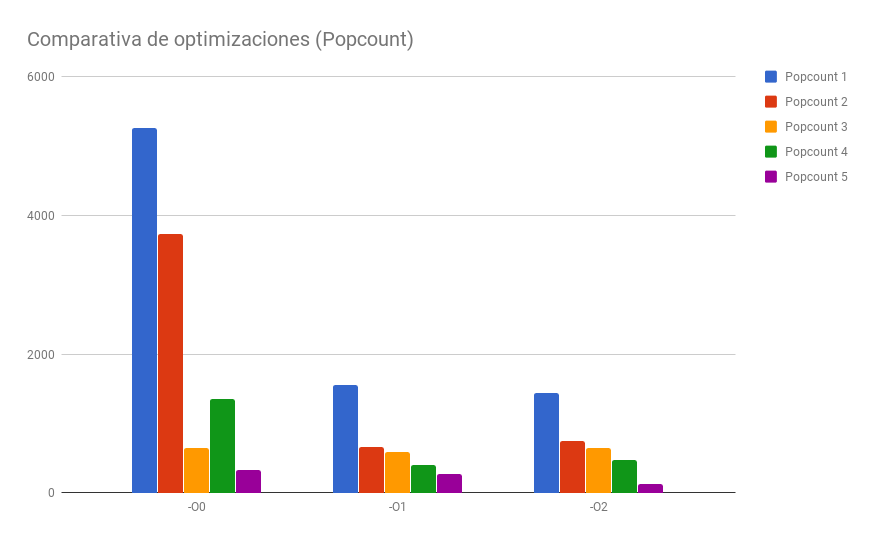
\includegraphics[width=1.1\textwidth]{popcount.png}
\end{figure}

\newpage

\subsection*{Parity}

\begin{flushleft}
  Tras haber realizado mediciones de tiempo a las distintas funciones
  programadas en el archivo \textit{parity.c} los resultados fueron los
  siguientes:
\end{flushleft}

\begin{table}[!htbp]
\centering
\caption{Parity -O0}
\label{my-label}
\begin{tabular}{|l|l|l|l|l|l|l|l|l|l|l|l|}\hline
-O0      & 0    & 1    & 2    & 3    & 4    & 5    & 6    & 7    & 8    & 9    & Media \\\hline
Parity 1 & 6205 & 5642 & 5385 & 5219 & 5181 & 5112 & 5607 & 5518 & 6726 & 5110 & 5571  \\\hline
Parity 2 & 2845 & 2144 & 2174 & 2206 & 2738 & 2155 & 2223 & 2279 & 2773 & 2138 & 2368  \\\hline
Parity 3 & 2634 & 1898 & 1917 & 1955 & 2076 & 1886 & 1947 & 2487 & 2327 & 2028 & 2116  \\\hline
Parity 4 & 1140 & 738  & 668  & 693  & 1011 & 671  & 697  & 703  & 826  & 969  & 812   \\\hline
Parity 5 & 1021 & 908  & 825  & 852  & 967  & 820  & 1067 & 842  & 1009 & 1344 & 966   \\\hline
Parity 6 & 218  & 223  & 195  & 202  & 203  & 196  & 202  & 202  & 241  & 286  & 217   \\\hline
\end{tabular}
\end{table}

\begin{table}[!htbp]
\centering
\caption{Parity -O1}
\label{my-label}
\begin{tabular}{|l|l|l|l|l|l|l|l|l|l|l|l|}\hline
-O1      & 0    & 1    & 2    & 3    & 4    & 5    & 6    & 7    & 8    & 9    & Media \\\hline
Parity 1 & 3960 & 1365 & 1373 & 1525 & 1575 & 1348 & 1357 & 1345 & 1335 & 2574 & 1776  \\\hline
Parity 2 & 1885 & 669  & 637  & 1161 & 743  & 637  & 637  & 637  & 637  & 784  & 843   \\\hline
Parity 3 & 1914 & 657  & 684  & 824  & 756  & 696  & 657  & 657  & 658  & 834  & 834   \\\hline
Parity 4 & 2589 & 636  & 637  & 1017 & 728  & 637  & 637  & 636  & 637  & 783  & 894   \\\hline
Parity 5 & 381  & 349  & 350  & 467  & 399  & 349  & 349  & 350  & 349  & 430  & 377   \\\hline
Parity 6 & 56   & 55   & 55   & 62   & 63   & 55   & 54   & 55   & 55   & 68   & 58    \\\hline
\end{tabular}
\end{table}

\begin{table}[!htbp]
\centering
\caption{Parity -O2}
\label{my-label}
\begin{tabular}{|l|l|l|l|l|l|l|l|l|l|l|l|}\hline
-O2      & 0    & 1    & 2    & 3    & 4    & 5    & 6    & 7    & 8    & 9    & Media \\\hline
Parity 1 & 2527 & 1429 & 1417 & 1508 & 1495 & 1495 & 1750 & 1549 & 1549 & 1393 & 1611  \\\hline
Parity 2 & 545  & 530  & 463  & 483  & 483  & 495  & 568  & 531  & 619  & 531  & 525   \\\hline
Parity 3 & 371  & 371  & 371  & 408  & 397  & 472  & 559  & 437  & 374  & 370  & 413   \\\hline
Parity 4 & 679  & 710  & 681  & 761  & 725  & 725  & 764  & 751  & 682  & 668  & 715   \\\hline
Parity 5 & 281  & 279  & 282  & 300  & 300  & 295  & 305  & 311  & 287  & 273  & 291   \\\hline
Parity 6 & 57   & 57   & 57   & 61   & 61   & 61   & 62   & 62   & 55   & 55   & 59   \\\hline
\end{tabular}
\end{table}

\newpage
En la siguiente gráfica hemos representado los resultados obtenidos:

\begin{figure}[!htbp]
  \centering
  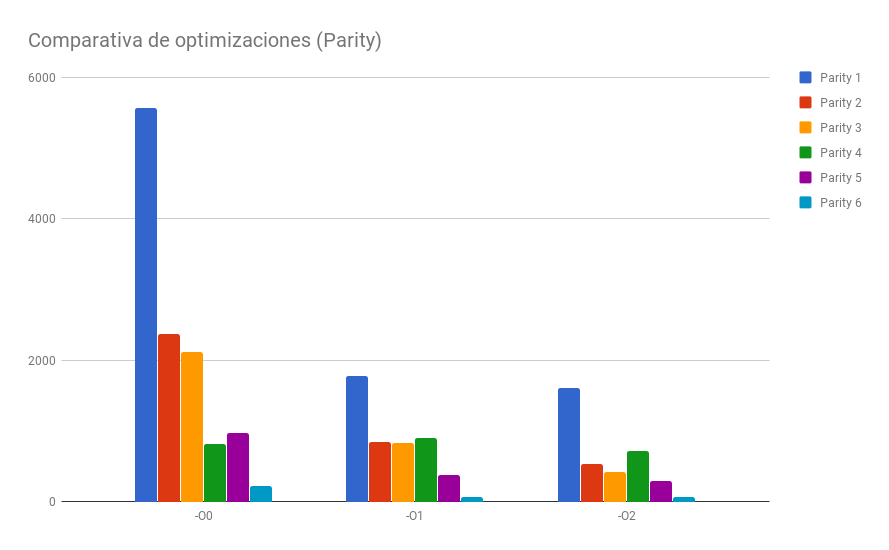
\includegraphics[width=1.1\textwidth]{parity.png}
\end{figure}


\end{document}